\begin{figure}[H]
\centering
% ---- (a) Loss ----
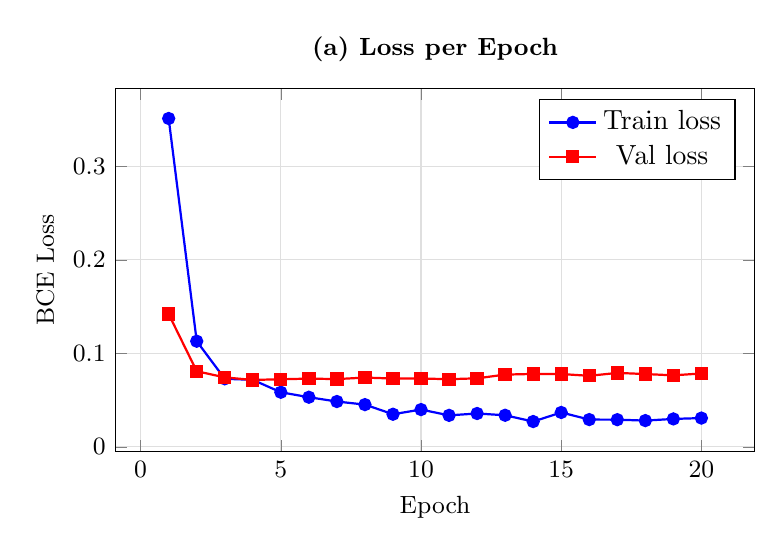
\begin{tikzpicture}
\begin{axis}[
    width=0.8\linewidth, height=6.2cm,
    title={\textbf{(a) Loss per Epoch}},
    xlabel={Epoch}, ylabel={BCE Loss},
    legend pos=north east, grid=both,
    grid style={gray!25}, tick label style={font=\small},
    label style={font=\small}, title style={font=\small\bfseries},
]
\addplot[blue, mark=*, thick] coordinates {(1,0.3512) (2,0.113) (3,0.0728) (4,0.0717) (5,0.0584) (6,0.0531) (7,0.0485) (8,0.0452) (9,0.0349) (10,0.0399) (11,0.0337) (12,0.0357) (13,0.0338) (14,0.0271) (15,0.0368) (16,0.0292) (17,0.0291) (18,0.0281) (19,0.0299) (20,0.0308)};
\addlegendentry{Train loss}
\addplot[red, mark=square*, thick] coordinates {(1,0.142) (2,0.0809) (3,0.0743) (4,0.0716) (5,0.0723) (6,0.073) (7,0.0725) (8,0.0741) (9,0.0731) (10,0.0731) (11,0.0724) (12,0.0733) (13,0.0773) (14,0.078) (15,0.0779) (16,0.076) (17,0.0791) (18,0.0779) (19,0.0765) (20,0.0785)};
\addlegendentry{Val loss}
\end{axis}
\end{tikzpicture}

\vspace{0.6em}
% ---- (b) F1 / AUC ----
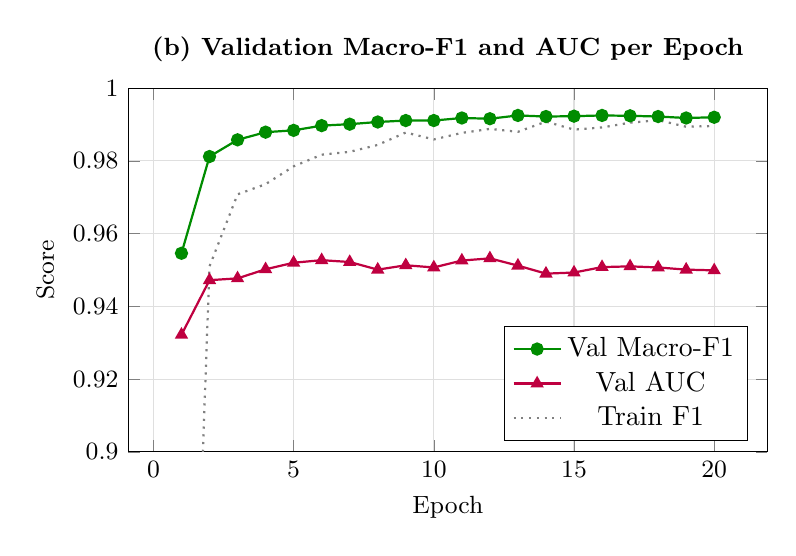
\begin{tikzpicture}
\begin{axis}[
    width=0.8\linewidth, height=6.2cm,
    title={\textbf{(b) Validation Macro-F1 and AUC per Epoch}},
    xlabel={Epoch}, ylabel={Score},
    ymin=0.9, ymax=1.0,
    legend pos=south east, grid=both,
    grid style={gray!25}, tick label style={font=\small},
    label style={font=\small}, title style={font=\small\bfseries},
]
\addplot[green!55!black, mark=*, thick] coordinates {(1,0.9546) (2,0.9812) (3,0.9858) (4,0.9879) (5,0.9884) (6,0.9897) (7,0.9901) (8,0.9907) (9,0.9911) (10,0.9911) (11,0.9918) (12,0.9916) (13,0.9925) (14,0.9922) (15,0.9923) (16,0.9925) (17,0.9924) (18,0.9922) (19,0.9918) (20,0.992)};
\addlegendentry{Val Macro-F1}
\addplot[purple, mark=triangle*, thick] coordinates {(1,0.9322) (2,0.9472) (3,0.9477) (4,0.9502) (5,0.952) (6,0.9527) (7,0.9522) (8,0.9501) (9,0.9513) (10,0.9507) (11,0.9526) (12,0.9532) (13,0.9512) (14,0.949) (15,0.9493) (16,0.9508) (17,0.951) (18,0.9507) (19,0.9501) (20,0.9499)};
\addlegendentry{Val AUC}
\addplot[gray, dotted, thick] coordinates {(1,0.736) (2,0.951) (3,0.9708) (4,0.9736) (5,0.9785) (6,0.9817) (7,0.9825) (8,0.9844) (9,0.9878) (10,0.9859) (11,0.9877) (12,0.9888) (13,0.988) (14,0.9908) (15,0.9886) (16,0.9892) (17,0.9905) (18,0.9912) (19,0.9894) (20,0.9896)};
\addlegendentry{Train F1}
\end{axis}
\end{tikzpicture}
\caption[Stage 1 training curves]{Stage~1 training dynamics. (a) Train and
validation BCE loss per epoch. (b) Validation macro-F1 (peak 0.9925) and AUC,
with train F1 for reference. The model converges within a few epochs and the
small train--validation gap indicates minimal overfitting.}
\label{fig:stage1_curves}
\end{figure}
